\begin{figure}[t]
\centering
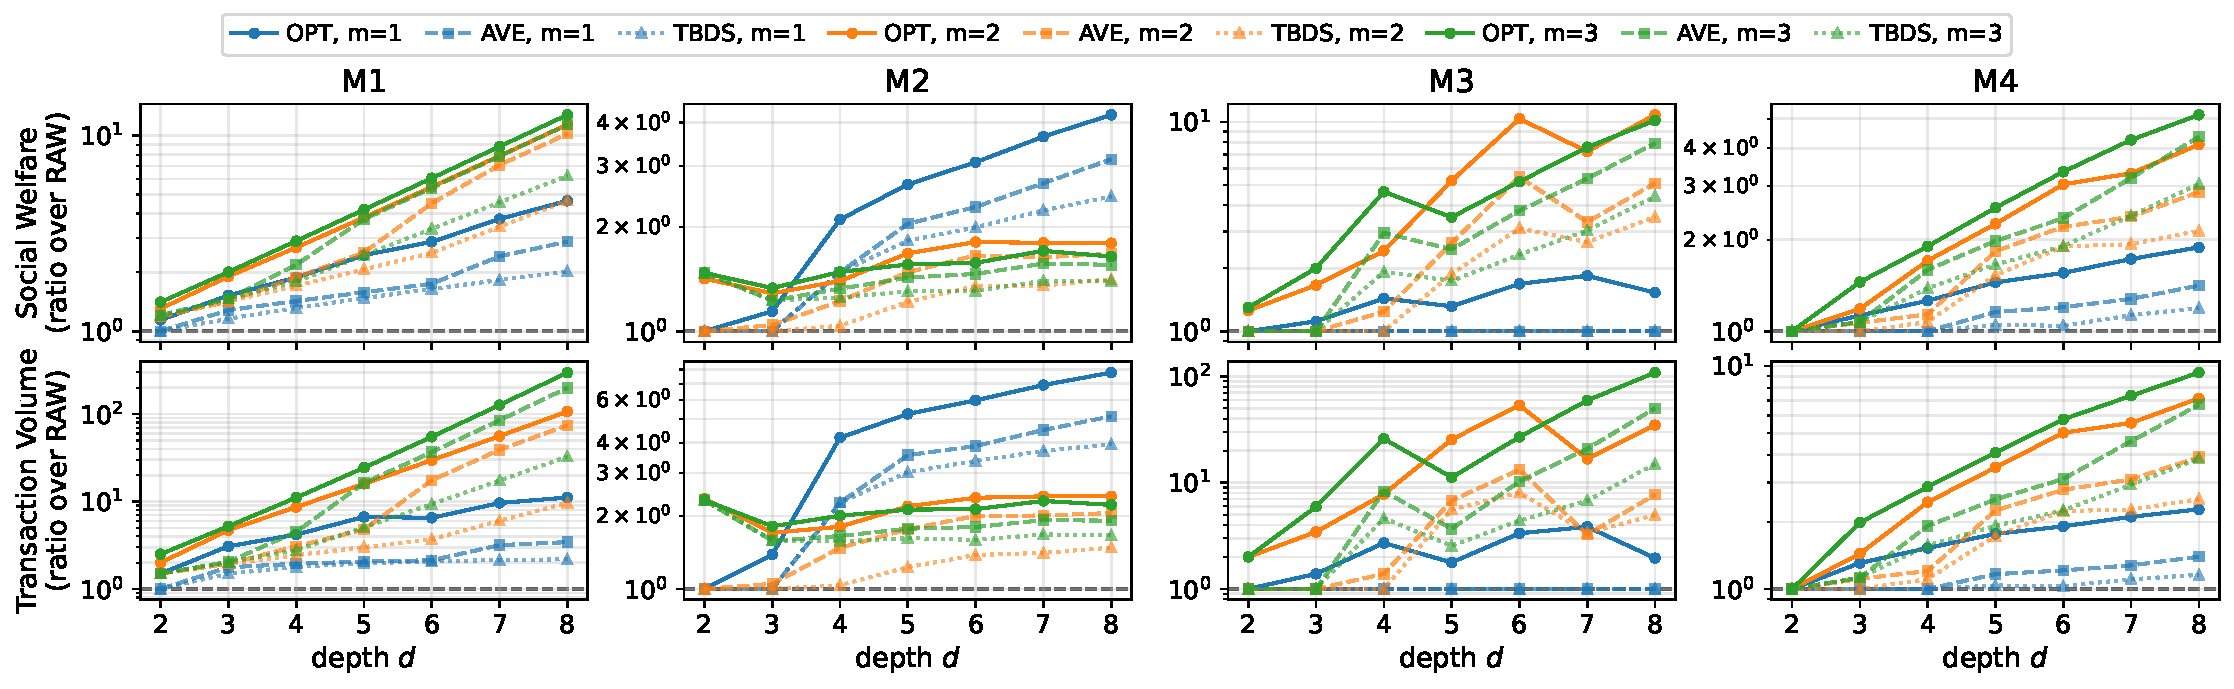
\includegraphics[width=\textwidth]{Materials/exp_vary.pdf}
\caption{Equilibrium social welfare (top) and transaction volume (bottom) of the AVE and OPT mechanisms, expressed as a ratio over the baseline RAW mechanism, as the tree depth $d$ varies from $2$ to $8$. Each column is one valuation model; colors denote the branching factor $m \in \{1,2,3\}$ ($m=1$ is the chain). Ratios above the dotted line ($=1$) indicate that profit reallocation improves upon the baseline. The advantage generally grows with depth and branching.}
\label{fig:exp-vary}
\end{figure}
